\begin{figure}
    \begin{center}
    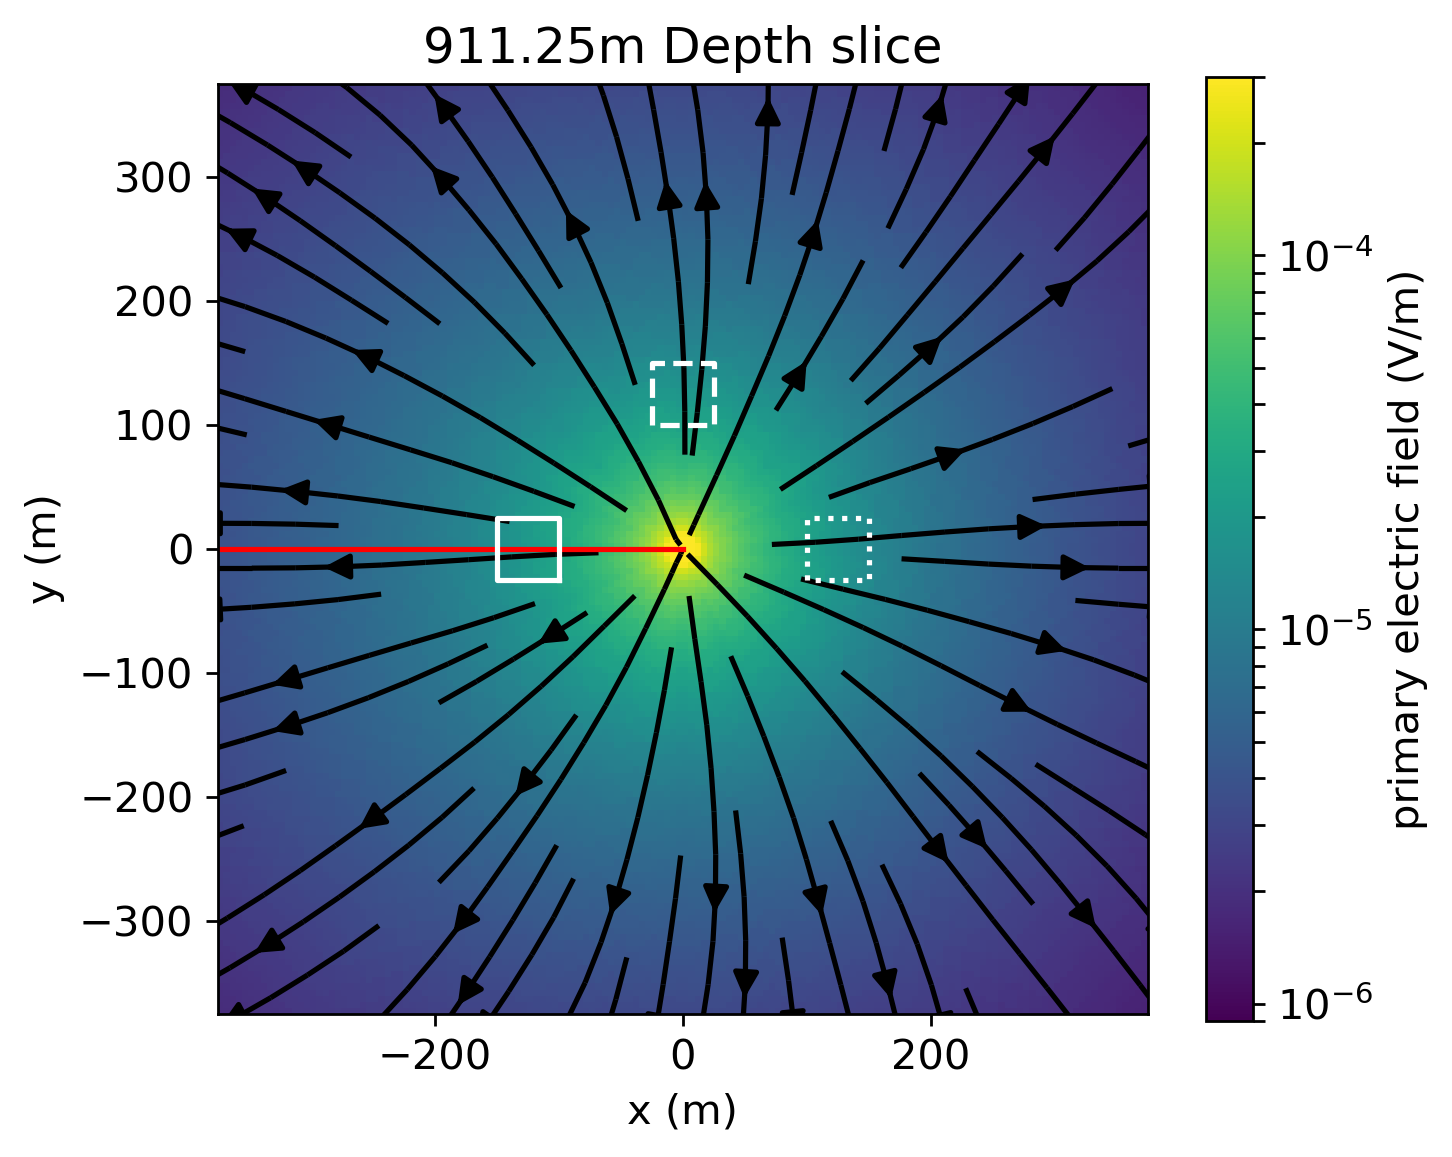
\includegraphics[width=0.6\textwidth]{figures/primary_3D.png}
    \end{center}
\caption{
    Depth slice showing the primary electric field due to a downhole
    electrode and a return electrode located on the surface at x=-500m, y=0m. The red line indicates the
    azimuth of the source.
    We examine the 3 different target azimuths shown by the white outlines.
    The solid line indicates the target inline with the source,
    the dashed is $90^\circ$ from the source line, and the dotted line is $180^\circ$ from the source line.
}
\label{fig:primary_3D}
\end{figure}
